
\section{Cooling System} 
\subsection{Overview}
\subsubsection{Requirements and Constraints}
The cooling system plays a pivotal role in keeping the motor, battery, and traction controller within safe temperature limits. Overheating can lead to reduced efficiency and potentially shorten the lifespan of these components. For instance, excessive heat could cause bearings to wear out faster, damage motor windings, and even demagnetize permanent magnets. Given the hyperloop's low-pressure environment, we must think beyond standard air cooling methods. Consequently, the exploration of alternative cooling techniques, such as liquid cooling, cooling with the Phase Changing Materials are becoming imperative for ensuring the system's reliability and efficiency.

\subsubsection{Estimated Cost and Part List}
The total estimated manufacturing cost for the cooling system is approximately 1200 Euros, considering the primary components outlined in the table. Despite its comprehensive functionality, the system maintains a relatively lightweight and compact profile, comprising only a select few components. This cost-effective design approach ensures efficient performance without compromising on reliability or functionality.


\autoref{table:components}
\begin{table} [H]
\centering
\caption{Components and Manufacturing Details}
\label{table:components}
\begin{adjustbox}{width=\textwidth,center}
\begin{tabular}{|>{\bfseries}m{2.9cm}|m{2.4cm}|m{1.7cm}|m{2.5cm}|m{2.2cm}|m{2.6cm}|m{2.2cm}|}
\hline
Component & Number & Mass [kg] & Size [mm] & Material & Manufacturing process & In-house/ Outsourced \\
\hline
Heat Exchanger & x1 & 1.1 & 100 x120 x100 & Aluminum & LPBF Printing & in-house \\
Drain Valve & x1 & 0.02 & M8 & Aluminum & Latheturning & in-house \\
PCM & x1.75 [liters] & 2 & - & PCM & - & outsourced \\
Deionized Water & x3 [liters] & 3 & - & Water & - & outsourced \\
Coolant Pump & x1 &1.2 & - & - & - & outsourced \\
Filter &x1 & 0.1 & - & - & - &outsourced \\
Coolant Temperature Sensor & x2 & 0.2 & - & - & - & outsourced \\
Surface Temperature Sensor & x3 & 0.2 & - & - & - & outsourced \\
Flow Meter & x1 & 0.1 & - & - & - & outsourced \\
Pressure Sensor & x4 & 0.1 & - & - & - & outsourced \\
Piping & x5 [meters] & 0.9 &  10 x 16& - & - & outsourced \\
Piping & x2 [meters] & 0.4 & 20 x 26 & - & - & outsourced \\
Tank & x1 & 0.2 & 138 x 160 & - & - & outsourced \\

Fittings & x15 & - & - & - & - & outsourced \\
\hline
\end{tabular}
\end{adjustbox}
\end{table}


\subsection{Objectives, Design process, and Cooling Requirements}
\autoref{fig:Cooling system}
\begin{figure}[ht]
  \centering
  \subfloat[Front view of the pod]{
    \centering
    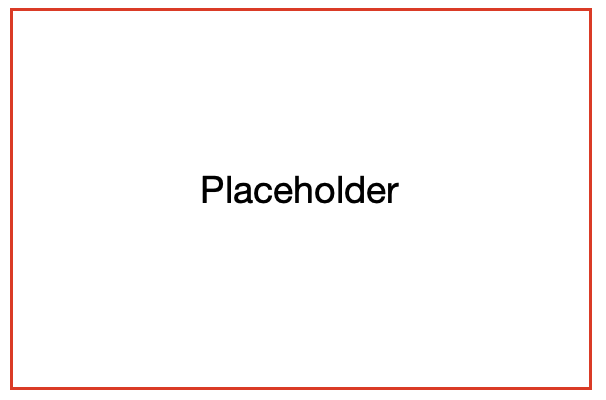
\includegraphics[width=0.5\linewidth]{texfiles/mech/eimg/cooling/placeholder}
    \label{fig:Front view}
  }
  \subfloat[Top view of the pod]{
    \centering
    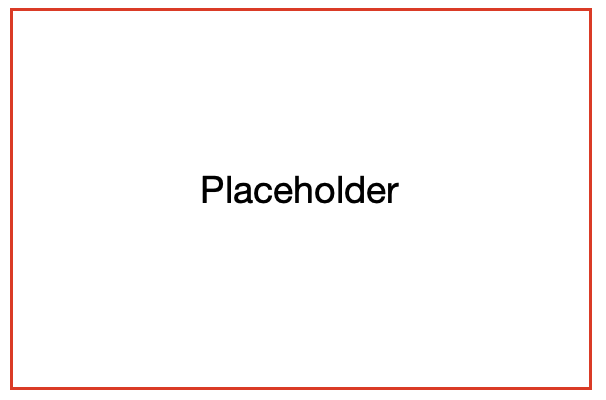
\includegraphics[width=0.5\linewidth]{texfiles/mech/eimg/cooling/placeholder}
    \label{fig:Top view}
  }
  \caption{Placement of the Cooling system}
  \label{fig:Cooling system}
\end{figure}


\subsubsection{ Motor}
The EMRAX motor is required to operate within a temperature range of -40°C to 120°C for both the copper windings and magnets. To safeguard against overload, a temperature sensor is integrated into the motor and must be linked to the controller. If the temperature surpasses the permissible limit, the controller adjusts the motor's current output to lower levels until the temperature stabilise within the acceptable range, with a worst-case motor efficiency of 92\%, approximately 4.8 kW of heat is generated during operation.

The manufacturer recommends a coolant flow rate of 6 to 8 litres per minute, with the coolant maintained at a maximum temperature of 50°C when entering the motor. Additionally, ambient air temperature surrounding the motor should ideally be 25°C or lower. [Ref - Product Spec Emrax Motor]


\subsubsection{ Traction Controller}

According to the product specification, the maximum permissible temperature for the traction controller is 150°C. However, to guarantee peak performance and longevity, it's essential to maintain temperatures below 90°C. After assessing the operating current and internal resistance, the estimated heat generation was calculated to be 0.56 kW. Through heat transfer calculations from the power module baseplate, equipped with fins, to the coolant, a water flow rate of 0.7 litres per minute was determined necessary to sustain the traction controller's temperature at 90°C.This ensures optimal cooling performance and contributes to the longevity and efficiency of the entire cooling system.
\subsubsection{ Battery}
The battery system within the hyperloop pod generates approximately 3.84 kW of heat during operation. This heat generation is primarily due to internal resistance within the battery cells as electrical energy is converted into usable power. To maintain safe and efficient operation, it is imperative to ensure that the temperature of the battery remains below 75°C.

When a battery operates at elevated temperatures, several detrimental effects may occur. High temperatures can accelerate the degradation of battery components, including the electrolyte and electrode materials, leading to reduced battery capacity and lifespan. Additionally, overheating increases the risk of thermal runaway, a phenomenon where the battery temperature rapidly increases, potentially resulting in fire or explosion.


\subsubsection{Cooling Requirements and Strategies}
To mitigate these risks and ensure the longevity and safety of the battery system, effective cooling strategies are essential. This includes implementing cooling systems, such as liquid cooling or cooling plates, to dissipate the heat generated by the battery during operation.

To ensure optimal cooling for all three vital components, the system necessitates a total coolant volume of 1 liters of de-ionised water. This calculation factors in the total heat generation (9.2 kW), the duration of a single run at the European Hyperloop Week Competition (20 seconds), and a safety factor of 3 (total time 60 seconds). After 60 seconds of operation, the maximum temperature of the 3 liters of coolant reaches approximately 66.5°C, well below the specified temperature limits. Further analysis during testing phase will provide valuable insights into coolant temperature changes and component temperatures.

To enhance the cooling performance of the cooling System, a refined hardware architecture will be implemented. Temperature levels play a critical role in determining the durability and efficiency of the motor, battery, and traction controller within the hyperloop pod. Elevated temperatures can adversely affect various components, including bearings, motor windings, and permanent magnets, potentially leading to demagnetisation. Therefore, prioritising the enhancement of cooling systems is essential for achieving significant long-term cost savings and improved performance. Given the impracticality of air cooling in the low-pressure hyperloop tube environment, alternative approaches such as liquid cooling and the use of Phase changing materials must be explored.

\subsubsection{Hardware Architecture for Enhanced Cooling}

As illustrated in  figure ~\ref{fig:schematic}, cold water stored at room temperature (approximately 20-25°C) will undergo filtration and then be pumped into the water jackets of the motor, traction controller, and battery in a closed-loop configuration, with a flow rate ranging from 8 to 12 liters per minute. Continuous monitoring of the coolant, motor, traction controller, and battery temperatures will be conducted. Should the temperature of any component exceed the specified limit, the control system will promptly deactivate the pod's drive motor.

Given the absence of heat transfer with the atmosphere during operation, the coolant temperature will gradually increase. Consequently, it's imperative that the coolant within the system remains below the temperature limits of each component. Cooling down the coolant prior to the pod's subsequent operation will be necessary.s
Pressure sensors have been strategically positioned at designated locations, as depicted in the diagram, to accurately gauge pressure drops across the water jackets during the testing phase. This data will be instrumental in fine-tuning the system's performance and ensuring optimal cooling efficiency.

\subsection{Appearance and Integration}
\subsubsection{Coolant }
Deionized water has been selected as the primary coolant for the system due to its low electrical conductivity. This choice is paramount in minimising the potential adverse effects of coolant leaks on the pod's electronic components. Although glycol is a common coolant choice in many cooling systems, it is not utilized in this particular system. This decision is attributed to the fact that the operating temperatures within the system consistently remain well above the freezing point of water, rendering glycol unnecessary.
\subsubsection{Coolant Pump}
During the testing phase, the Rheinmetall WUP 25 pump will serve as the primary pump for the cooling system. Although typically employed in the realm of combustion engines and vehicle climate control systems, the WUP 25 pump demonstrates versatility by effectively handling various cooling tasks, including cooling DC/DC converters, batteries, electric motors, and power electronics. Its compact design allows for installation in constrained spaces, and it offers a range of hydraulic and electrical interfaces to suit diverse applications. Equipped with a control and diagnostic pin, the WUP 25 pump facilitates speed control via a PWM input signal [Ref = Product Data Sheet WUP 25]. 

To ensure optimal performance, the pump will be mounted at a mid-level position within the cooling circuit. This strategic placement helps prevent the formation of air traps (if mounted at the highest position) and minimizes the risk of debris accumulation within the pump (if mounted at the lowest position) [Ref = Product Data Sheet WUP 25]. However, due to the current uncertainty regarding the pressure drop in the system, it may be necessary to explore alternative pump options or implement a multi-stage pump system (in series) alongside the existing model. The exact pressure drop across the water jackets will be determined through rigorous testing
\begin{figure}[ht]
  \centering
  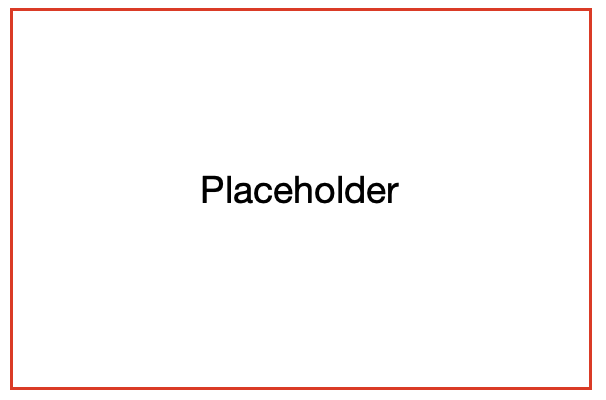
\includegraphics[width=0.5\linewidth]{texfiles/mech/eimg/cooling/placeholder}
  \caption{Coolant pump}
  \label{fig:Coolant Pump}
\end{figure}

\subsubsection{Coolant Storage Tank}
The cooling system is designed with consideration for the realistic scenario of the pod traveling through a low-pressure tube (near vacuum), limiting heat exchange with the atmosphere. The coolant in the circuit absorbs heat from the motor, battery, and traction controller, causing an increase in coolant temperature over time. The current design ensures sufficient coolant storage to keep all components well below the required maximum operating temperature.

For the hyperloop pod slated for participation in the European Hyperloop Week, a typical vehicle coolant tank with a capacity of 1 liter has been deemed adequate. This capacity aligns with the demands of the pod's cooling requirements, guaranteeing optimal performance throughout its operation.
\begin{figure}[ht]
  \centering
  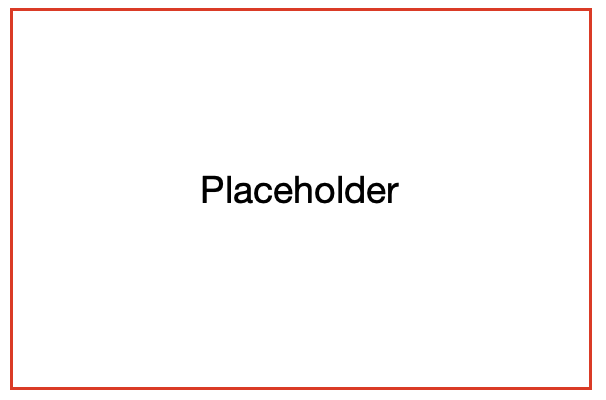
\includegraphics[width=0.5\linewidth]{texfiles/mech/eimg/cooling/placeholder}
  \caption{Coolant tank}
  \label{fig:Coolant tank}
\end{figure}

\subsubsection{Water Jackets}
The water jacket for the motor will be provided by the motor manufacturer, ensuring compatibility and optimal performance. For the water jackets of the traction controller and battery, custom fabrication will be undertaken based on the recommendations provided by their respective manufacturers. This approach guarantees that each component receives tailored cooling solutions to meet its specific requirements and operating conditions.

\subsubsection{Piping}
Two piping options are under consideration.
 i) CPVC pipes, chosen for their resistance to high temperatures, scaling, durability, low cost, and ease of installation. The specific piping route is yet to be finalized , but the total length is estimated to be around 6 meters. 
ii) The potential use of soft tubing is also being explored.

\subsection{Heat Exchanger}
\subsubsection{Role and Benefits in the cooling System}
In the context of the cooling system described for the hyperloop pod, a heat exchanger would play a crucial role in transferring heat between the coolant circulating within the closed-loop system and the surrounding environment. As the coolant circulates through the system, it absorbs heat from the motor, battery, and traction controller, thereby increasing in temperature. Since the hyperloop pod operates in a low-pressure tube with limited heat exchange with the atmosphere, the heat exchanger facilitates the dissipation of heat even in this constrained environment.

\begin{figure}[ht]
  \centering
  \subfloat[Closed View]{
    \centering
    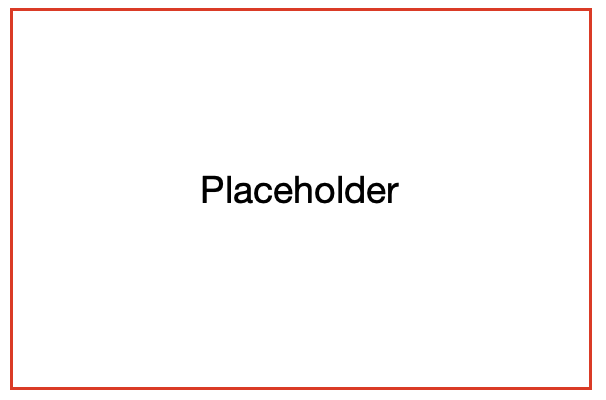
\includegraphics[width=0.5\linewidth]{texfiles/mech/eimg/cooling/placeholder}
    \label{fig:HE Closed view}
  }
  \subfloat[Open View]{
    \centering
    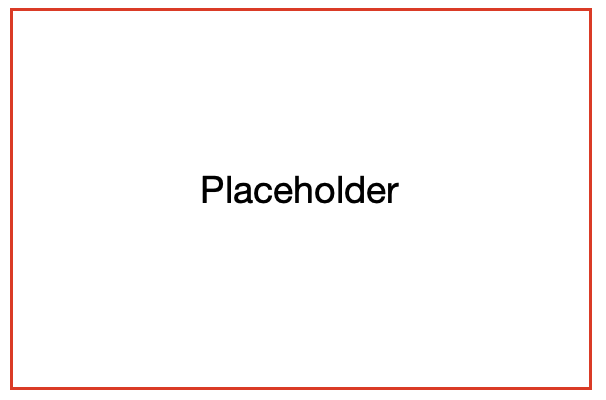
\includegraphics[width=0.5\linewidth]{texfiles/mech/eimg/cooling/placeholder}
    \label{fig:HE Open view}
  }
  \caption{Gyroid Heat Exchanger}
  \label{fig:HE}
\end{figure}


\subsubsection{Use of Phase Change Materials (PCMs)}
Introducing the heat exchanger utilizing phase change materials (PCMs) into the cooling system for the hyperloop pod would offer several advantages and could enhance its performance in specific scenarios, incorporating a heat exchanger with the use of phase changing material serves several important purposes:

\begin{itemize}
  \item \textbf{Enhanced Heat Absorption and Release:} The PCM, such as stearic acid, can absorb and release a significant amount of heat during its phase transition from solid to liquid and vice versa. Integrating a heat exchanger with PCM allows for efficient absorption of excess heat generated by components like the motor, traction controller, and battery.
  \item \textbf{Temperature Regulation:} By absorbing excess heat from critical components, the heat exchanger helps regulate their temperatures within the specified operating ranges. This prevents overheating, which can lead to performance degradation or damage to components.
  \item \textbf{Thermal Energy Storage:} The PCM's ability to store thermal energy during its phase change enables the system to store heat when temperatures are within acceptable limits and release it when needed to maintain optimal operating conditions. This helps in managing transient heat loads and stabilizing temperatures over time.
  \item \textbf{Reduced Coolant Temperature:} By utilizing the PCM's heat absorption capacity, the heat exchanger can lower the temperature of the coolant circulating in the system. This ensures that the coolant remains within acceptable temperature limits, contributing to the overall effectiveness of the cooling system.
  \item \textbf{Increased Efficiency:} Integrating a heat exchanger with PCM can improve the overall efficiency of the cooling system by maximizing heat transfer capabilities and reducing the reliance on conventional cooling methods alone.
  \item \textbf{Extended Operating Time:} The thermal energy stored in the PCM can be utilized to extend the operating time of the system before coolant temperature rises beyond acceptable levels. This can be particularly beneficial during transient operating conditions or in the event of temporary power interruptions.
\end{itemize}

Overall, incorporating a heat exchanger with the use of phase changing material adds an additional layer of heat management capability to your cooling system, contributing to improved performance, efficiency, and reliability in the hyperloop pod environment.


\subsubsection{Stearic Acid}

Stearic acid stands out as a highly versatile phase change material (PCM) deployed across diverse applications. Its unique characteristic of transitioning from solid to liquid state at a precise temperature renders it exceptionally suitable for thermal energy storage purposes. Through this phase transition, stearic acid exhibits remarkable heat absorption and release capabilities, making it a valuable asset in scenarios demanding efficient temperature regulation and thermal energy management. Commonly found in applications ranging from building insulation to specialized temperature control systems, stearic acid's efficacy as a PCM underscores its widespread industrial utility.

\paragraph{Stearic Acid}
Stearic acid is a saturated fatty acid with the chemical formula \( C_{18}H_{36}O_2 \). It is a long-chain carboxylic acid, meaning it has 18 carbon atoms in its hydrocarbon chain and a carboxyl group (COOH) at one end. Here are some key properties and uses of stearic acid:

\subparagraph{Physical Properties:}
\begin{itemize}
  \item Melting Point: Stearic acid is a solid at room temperature and has a melting point of around \( 69-70 \) degrees Celsius (\( 156-158 \) degrees Fahrenheit).
  \item Appearance: It is a white, waxy solid with a characteristic fatty odor.
\end{itemize}

\subparagraph{Chemical Properties:}
\begin{itemize}
  \item Structure: Stearic acid has a straight-chain structure with 18 carbon atoms, making it a saturated fatty acid. Hydrophobic: Like other fatty acids, stearic acid is hydrophobic, meaning it repels water.
\end{itemize}

In summary, stearic acid is a versatile compound with various industrial applications, and its phase change properties make it useful in thermal energy storage applications as well.

\subsection{Calculations and Simulations}

\textbf{WILL BE ADDED SOON (Dino)}
\subsection{Safety Measures}
Given the close integration of the cooling system with the electronic systems, the primary risk is a coolant leak that could potentially damage electronic components. Preventive measures are outlined in the table below, and deionised water is chosen as the preferred coolant due to its low conductivity.
\subsubsection{Potential Failure Modes and Risk Mitigation-}
\begin{itemize}
  \item \textbf{Coolant Leaks}
    \begin{itemize}
      \item Effect of Failure: Damage Electronic components
      \item Root Cause: Poor sealing at pipe joints
      \item Risk Mitigation Strategy: Maintain the correct coolant level, avoid overfilling the tank, sealing pipes with hose clamps and use deionized water as a coolant.
    \end{itemize}
  \item \textbf{Temperature of Critical component rises above rated temperature}
    \begin{itemize}
      \item Effect of Failure: Damage Component
      \item Root Cause: Insufficient cooling due to prolonged operation
      \item Risk Mitigation Strategy: Implement a control system to halt the motor and by installing two temperature sensors if temperatures exceed prescribed limits for the motor, battery, or traction controller.
    \end{itemize}
  \item \textbf{Temperature of Critical component rises above rated temperature}
    \begin{itemize}
      \item Effect of Failure: Coolant Leaks
      \item Root Cause: Insufficient cooling due to air traps or exceeding defined operation time
      \item Risk Mitigation Strategy: Position of the system including heat exchanger is placed at the front of the pod, in order to purge air after refilling, and adhere to defined operation times.
    \end{itemize}
  \item \textbf{Blocks in piping}
    \begin{itemize}
      \item Effect of Failure: Insufficient cooling and damage to components
      \item Root Cause: Foreign particles/debris
      \item Risk Mitigation Strategy: Introduce filters in the piping system and conduct regular cleaning maintenance.
    \end{itemize}
\end{itemize}


\subsubsection{FMEA analysis}

\subsubsection{References}

\begin{figure}[ht]
  \centering
  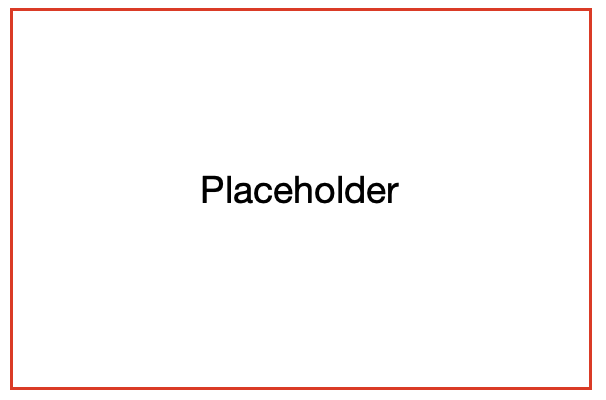
\includegraphics[width=\linewidth]{texfiles/mech/eimg/cooling/placeholder}
  \caption{Flowchart of the system}
  \label{fig:schematic}
\end{figure}




